\documentclass[../../main]{subfiles}

\begin{document}
\chapter{数ベクトル空間}
\label{chapter:numerical_vector_space}

\begin{lead}
  \cref{chapter:numerical_vector_space}で書く予定のことを並べておく.
\end{lead}

\section{行列とベクトル空間}
信号解析に関連する議論へと移る前に,有限次元の線型代数について簡単に説明しておく.

\subsection{基底}
任意のベクトル\(\vect{x}=\trps{\inlinevec{x_1 & \cdots & x_n}}\in\numset{K}^n\)は,第\(i\)成分が\(1\),他の成分が\(0\)のベクトル\(\vect{e}_i\)を用いて
\(\vect{x}=x_1\vect{e}_1+\dots+x_n\vect{e}_n\)と表せる.
すなわち,集合\(\basis{B}_n=\Set{\vect{e}_1,\dots,\vect{e}_n}\)は「\(\numset{K}^n\)のすべての元を\(\basis{B}_n\)の元の線型結合で書ける」という性質を持つ.

一般に,ベクトル空間\(V\)の部分集合\(S\)に対して,\(S\)の元の線型結合で書けるベクトルの全体集合を\(S\)が\termdef{生成する部分空間}\index{ぶぶんくうかん@部分空間!せいせいする@生成する---}(generated subspace)といい,
\(\spannedby S\)\index{\(\spannedby S\)}と表記する.この記法を使えば,先述した\(\basis{B}_n\)が持つ性質を「\(\spannedby\basis{B}_n=\numset{K}^n\)が成り立つ」と言い換えられる.

\(\spannedby S=\numset{K}^n\)を満たす集合\(S\subset\numset{K}^n\)は,\(\basis{B}_n\)以外にも無数にある.
たとえば\(\numset{K}^n=\numset{R}^2\)のとき,集合\(T=\Set{\trps{\inlinevec{1 & 1}},\trps{\inlinevec{2 & -1}},\trps{\inlinevec{-1 & 0}}}\)が生成する部分空間は
\(\numset{R}^2\)である.しかし,\(\basis{B}_2=\Set{\trps{\inlinevec{1 & 0}},\trps{\inlinevec{0 & 1}}}\)の元の線型結合で\(\numset{R}^2\)の元を表す方法はただ1通りであるのに対して,\(T\)はこの性質を持たない(\cref{figure:linear_comb}).

\begin{figure}[htbp]
  \centering
  \begin{minipage}{\linewidth/2}
    \centering
    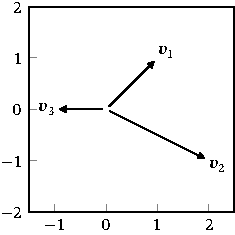
\includegraphics{linear_comb1.pdf}
  \end{minipage}%
  \begin{minipage}{\linewidth/2}
    \centering
    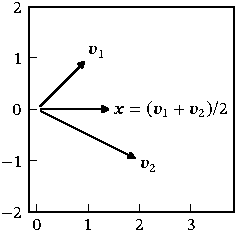
\includegraphics{linear_comb2.pdf}    
  \end{minipage}
  \caption{\(T\)の元の線型結合で\(\vect{x}=\trps{[\begin{matrix}3/2 & 0\end{matrix}]}\)を表した様子.明らかに\(\vect{x}=(-3/2)\vect{v}_3\)である一方,\(\vect{x}=(\vect{v}_1+\vect{v}_2)/2=(1/2)\vect{v}_1+(1/2)\vect{v}_2\)も成り立つ.}
  \label{figure:linear_comb}
\end{figure}

\(S\)の元の線型結合で\(\spannedby S\)の元を一意に表せるとき,任意の\(a_i,b_i\in\numset{K}\),\(\vect{v}_i\in S\)について
\begin{equation}
  \label{equation:span_uniqueness}
  \sum_{i=1}^ka_i\vect{v}_i = \sum_{i=1}^kb_i\vect{v}_i
  \implies (a_1,\dots,a_k) = (b_1,\dots,b_k)
\end{equation}
が成立する.\(c_i=a_i-b_i\)とおくと,\cref{equation:span_uniqueness}は
\begin{equation}
  \label{equation:independence}
  \sum_{i=1}^kc_i\vect{v}_i = \zvec
  \implies c_1 = \dots = c_k = 0
\end{equation}
と同値である.

任意の\(c_1,\dots,c_k\in\numset{K}\)に対して\cref{equation:independence}が成立するとき,
\(\vect{v}_1,\dots,\vect{v}_k\)は\termdef{線型独立}であるという.特に,\(V=\spannedby S\)かつ,\(S\)の元からなる有限個のベクトルの組が常に線型独立であるとき,\(S\)は\(V\)の\termdef{基底}であるという.
以上を\cref{definition:independence,definition:basis}にまとめておく.

\begin{definition}{生成系・線型独立・線型従属}{independence}
  \(V\)を\(\numset{K}\)上のベクトル空間,\(S\)を\(V\)の部分集合とする.
  \begin{enumerate}
    \item \(V=\spannedby S\)であるとき,\(S\)を\(V\)の\termdef{生成系}(generating set)という
    \item \(\vect{v}_1,\dots,\vect{v}_k\in V\)が\(\sum_{i=1}^kc_i\vect{v}_i=\zvec\implies c_1=\dots=c_k=0\)を満たすとき,
      \(\vect{v}_1,\dots,\vect{v}_k\)は\termdef{線型独立}\index{せんけいどくりつ@線型独立}(linearly independent)であるという
    \item \(\vect{v}_1,\dots,\vect{v}_k\in V\)が線型独立でないとき,\(\vect{v}_1,\dots,\vect{v}_k\)は\termdef{線型従属}\index{せんけいじゅうぞく@線型従属}(linearly dependent)であるという
  \end{enumerate}
\end{definition}

\begin{definition}{基底}{basis}
  \(V\)を\(\numset{K}\)上のベクトル空間,\(\basis{B}\)を\(V\)の部分集合とする.
  \(\basis{B}\)が\(V\)の生成系かつ,\(\basis{B}\)に属する有限個のベクトル\(\vect{v}_1,\dots,\vect{v}_k\)が常に線型独立であるとき,\(\basis{B}\)は\(V\)の\termdef{基底}\index{きてい@基底}(basis)であるという.
\end{definition}

\begin{example}[標準基底]
  \(\basis{B}_n\)は\(\numset{K}^n\)の基底である.\(\basis{B}_n\)を\(\numset{K}^n\)の\termdef{標準基底}\index{ひょうじゅんきてい@標準基底}(standard basis)という.
\end{example}

さきほどの議論によれば,\(S\)の元の線型結合で\(\spannedby S\)の元を一意に表せるとき,任意の\(c_1,\dots,c_k\in\numset{K}\)について\cref{equation:independence}が成立する.
すなわち,\(S\)は\(\spannedby S\)の基底である.実はこの逆も示せるので,次の命題が成立する.

\begin{proposition}{}{}
  \(V\)を\(\numset{K}\)上のベクトル空間,\(S\)を\(V\)の部分集合とする.このとき,次の命題は同値である.
  \begin{enumerate}
    \item \(S\)の元の線型結合で\(\spannedby S\)の元を一意に表せる
    \item \(S\)は\(\spannedby S\)の基底である
  \end{enumerate}
\end{proposition}

\(V\)の基底で有限集合のものがあるとき,\(V\)は\termdef{有限次元}\index{ゆうげんじげん@有限次元}(finite-dimensional)であるという.
\(V\)が有限次元なら,\(V\)の基底はすべて有限集合で,その元の個数は等しい.
すなわち,元の個数\(\sizeof{\basis{B}}\)は基底\(\basis{B}\)のとりかたによらず定まる.
\(\sizeof{\basis{B}}\)を\(V\)の\termdef{次元}\index{じげん@次元}(dimension)といい,\(\dim V\)\index{\(\dim V\)}と表記する
\footnote{\(V\)が有限次元でないときも基底は存在し,濃度は基底の選び方に依存しない(証明は文献\cite{yukie2019}).}.

\subsection{基底変換}
以下,\(V\)は有限次元であるとする.

\subsection{固有値と固有空間}
\begin{definition}{固有値,固有空間}{eigenvalue}\index{こゆうち@固有値}\index{こゆうべくとる@固有ベクトル}
\(\mat{A}\)を\(n\)次正方行列とする.
複素数\(\lambda\)と\(\zvec\)でないベクトル\(\vect{x}\in\numset{C}^n\)が式\(\mat{A}\vect{x}=\lambda\vect{x}\)を満たすとき,
\(\lambda\)を\(\mat{A}\)の\termdef{固有値}(eigenvalue)という.
また,\(\vect{x}\)を\(\mat{A}\)の(固有値\(\lambda\)に属する)\termdef{固有ベクトル}(eigenvector)という.
\end{definition}

\begin{definition}{固有空間}{eigenspace}\index{こゆうくうかん@固有空間}\index{\(E_\lambda(\mat{A})\)}
\cref{definition:eigenvalue}の\(\mat{A}\),\(\lambda\)について,集合
\[
  E_\lambda(\mat{A}) = \Set{\vect{x}\in\numset{C}^n\given\mat{A}\vect{x}=\lambda\vect{x}}
\]
は\(\numset{C}^n\)の部分空間になる.部分空間\(E_\lambda(\mat{A})\)を,
\(\mat{A}\)の(固有値\(\lambda\)に属する)\termdef{固有空間}(eigenspace)という.
\end{definition}

固有空間は次の性質を持つ.

\begin{proposition}{}{eigenspaces_disjointness}
\(\lambda_1\),\(\lambda_2\)を\(n\)次正方行列\(\mat{A}\)の固有値とする.
\begin{enumerate}
  \item \(\vect{x}\in E_{\lambda_1}(\mat{A})\implies\mat{A}\vect{x}\in E_{\lambda_1}(\mat{A})\)
  \item \(\lambda_1\neq\lambda_2\implies E_{\lambda_1}(\mat{A})\cap E_{\lambda_2}(\mat{A})=\Set{\zvec}\)
\end{enumerate}
\end{proposition}

\subsection{対角化}

\section{直交射影}
\subsection{直交射影}
\begin{figure}[htbp]
  \centering
  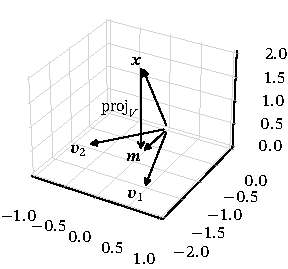
\includegraphics{projection.pdf}
\end{figure}

\subsection{直交補空間}
\subsection{スペクトル定理}

\section{最小二乗問題}
\subsection{最小二乗問題}
\subsection{特異値分解}
\subsection{擬似逆行列}

\section{離散フーリエ変換}

\section{多重解像度解析}

\begin{subappendices}
\section{主成分分析}
\begin{figure}[htbp]
  \begin{minipage}{\linewidth/2}
    \centering
    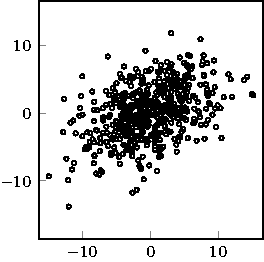
\includegraphics{scatter.pdf}
  \end{minipage}%
  \begin{minipage}{\linewidth/2}
    \centering
    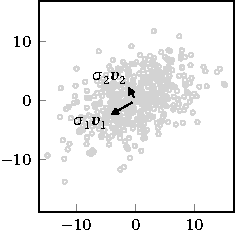
\includegraphics{pca.pdf}
  \end{minipage}
\end{figure}

\section{低ランク近似}
\section{窓関数}
\end{subappendices}

\section*{演習問題}
\addcontentsline{toc}{section}{演習問題}

\end{document}
